\documentclass[10pt,letterpaper]{article}
\usepackage[margin=0.7in]{geometry}
\usepackage[T1]{fontenc}
\usepackage{lmodern}
\usepackage{amsmath,amssymb,booktabs,graphicx,xcolor,hyperref}
\hypersetup{colorlinks=true,urlcolor=blue,linkcolor=blue,pdftitle={Foundations of Machine Learning and AI - Homework 1},pdfauthor={Ruochen Wang}}
\setlength{\parindent}{0pt}
\setlength{\parskip}{4pt}
\setlength{\emergencystretch}{2em}
\newcommand{\E}{\mathbb{E}}
\newcommand{\R}{\mathbb{R}}
\newcommand{\dd}{\mathrm{d}}
\newcommand{\code}[1]{\texttt{#1}}
\newcommand{\MSEExcess}{\ensuremath{3.35\times10^{-7}}}
\newcommand{\PredictionGap}{0.001148}
\newcommand{\TExcess}{\ensuremath{9.76\times10^{-8}}}
\newcommand{\StudentImprovement}{0.001322}
\newcommand{\StudentPercent}{0.68}

\begin{document}
\begin{center}
{\Large\bfseries Foundations of Machine Learning and AI}\\[4pt]
{\large Homework 1 \quad | \quad Fall 2026}\\[4pt]
{\large Ruochen Wang}
\\[4pt]
{\small \href{https://github.com/richard0525/foundations-machine-learning-ai}{Course GitHub repository}
\quad | \quad
\href{https://github.com/richard0525/foundations-machine-learning-ai/tree/main/homework_1}{Homework 1 code and results}}
\end{center}

\section*{1. Betting and expected utility}
Let $p=0.85$ be Victor's subjective probability and $q=0.60$ the market-implied
probability. Assume no fees, no borrowing, and an amount at risk $a\in[0,d]$.
Interpreting the market quote as a contract costing $q$ dollars and paying one
dollar if Biden wins, the net profit per dollar staked is
$b=(1-q)/q=2/3$. Final wealth is therefore
\[
W(a)=\begin{cases}d+ba,&\text{Biden wins},\\d-a,&\text{Biden loses}.\end{cases}
\]
\textbf{Wording ambiguity.} Literal ``even-money'' odds mean $b=1$, which conflicts
with $q=0.60$. The main solution uses the quoted probability; the literal
even-money alternative is given below.

\subsection*{(a) Linear utility}
For $U(W)=W$,
\[
\E[U(W(a))]=p(d+ba)+(1-p)(d-a)
=d+a\left(\frac{p}{q}-1\right)=d+\frac{5}{12}a.
\]
This is strictly increasing in $a$, so the unique optimum on $[0,d]$ is
$\boxed{a^*=d}$. The conclusion assumes the stake is capped at the bankroll;
otherwise positive expected profit could lead to unbounded borrowing in this
idealized model.

Linear utility represents risk neutrality: an additional dollar has the same
value regardless of current wealth. It can approximate preferences for small
stakes, but is usually implausible for an entire bankroll. It ignores diminishing
marginal utility and treats a 15\% chance of losing all wealth as acceptable
when expected wealth rises.

\subsection*{(b) Logarithmic utility}
For $0\le a<d$, define
\[
g(a)=p\log(d+ba)+(1-p)\log(d-a).
\]
Its derivatives are
\[
g'(a)=\frac{pb}{d+ba}-\frac{1-p}{d-a},\qquad
g''(a)=-\frac{pb^2}{(d+ba)^2}-\frac{1-p}{(d-a)^2}<0.
\]
Setting $g'(a)=0$ gives $pb(d-a)=(1-p)(d+ba)$ and thus
\[
\boxed{\frac{a^*}{d}=\frac{pb-(1-p)}{b}
=\frac{p-q}{1-q}=\frac{0.85-0.60}{0.40}=0.625.}
\]
Strict concavity makes this the unique maximum; $g(a)\to-\infty$ as $a\uparrow d$.
Under literal even-money odds, the same derivation gives
$a^*/d=2p-1=0.70$; part (a) still gives $a^*=d$.

\subsection*{(c) A hypothetical personal response}
No: I would not commit \$312,500 of a \$500,000 net worth to this one event.
At the quoted odds, final wealth would be approximately \$708,333 after a win and
\$187,500 after a loss. The calculation is optimal under the stated probability,
utility, and liquidity assumptions, but a probability estimate can be wrong,
net worth need not be liquid, and essential future spending may justify greater
risk aversion. Declining the full stake is consistent with changing these
assumptions; it does not invalidate part (b). This is a hypothetical judgment,
not a claim about an actual portfolio. With literal even-money odds, the proposed
stake would instead be \$350,000.

\newpage
\section*{2. Binary cross-entropy is a proper scoring rule}
Write $\eta(x)=P(Y=1\mid X=x)$ and let $f(x)\in[0,1]$ denote a predicted
probability. Binary cross-entropy is
\[
L(y,f(x))=-y\log f(x)-(1-y)\log(1-f(x)).
\]
Use the standard extended-value convention: a zero-probability term with zero
weight contributes zero, and an impossible positive-weight event has infinite loss.
Conditioning on $X=x$ gives
\[
r_x(u)=\E[L(Y,u)\mid X=x]
=-\eta(x)\log u-(1-\eta(x))\log(1-u).
\]
For $0<\eta(x)<1$ and $0<u<1$,
\[
r'_x(u)=-\frac{\eta(x)}u+\frac{1-\eta(x)}{1-u}
=\frac{u-\eta(x)}{u(1-u)},\qquad
r''_x(u)=\frac{\eta(x)}{u^2}+\frac{1-\eta(x)}{(1-u)^2}>0.
\]
The unique conditional minimizer is $u=\eta(x)$. At the boundaries,
$\eta(x)=0$ gives $r_x(u)=-\log(1-u)$, minimized at $u=0$;
$\eta(x)=1$ gives $r_x(u)=-\log u$, minimized at $u=1$.

By the tower property, global risk is $R(f)=\E_X[r_X(f(X))]$. More explicitly,
\begin{align*}
R(f)-R(\eta)
&=\E_X\!\left[
\eta(X)\log\frac{\eta(X)}{f(X)}
+(1-\eta(X))\log\frac{1-\eta(X)}{1-f(X)}\right]\\
&=\E_X\!\left[D_{\mathrm{KL}}\!\left(
\operatorname{Bern}(\eta(X))\,\Vert\,\operatorname{Bern}(f(X))\right)\right]\ge0.
\end{align*}
Equality holds precisely when $f(X)=\eta(X)$ almost surely. Thus binary
cross-entropy is \emph{strictly proper}, with probability vector
$f^*(x)=(1-\eta(x),\eta(x))$ if both class probabilities are reported.

This statement optimizes over all measurable probability predictors. A restricted
linear-logit model need not contain the true conditional probability. Also, a
finite sigmoid logit cannot attain 0 or 1, so in deterministic conditional cases
the optimum over finite logits is an infimum rather than an attained minimum.

\section*{3. Why a constant SGD step size can be reasonable}
The lecture's conditions $\sum_t\rho_t=\infty$ and $\sum_t\rho_t^2<\infty$
allow continued progress while asymptotically controlling persistent gradient
noise, alongside regularity assumptions. A finite dataset and
a finite training budget have a different goal: useful prediction, not arbitrarily
precise minimization of the empirical objective.

For a local scalar quadratic with curvature $h>0$, let the gradient noise
$\xi_t$ have mean zero and variance $\sigma_g^2$, independent across updates and
of the current error. Constant-step SGD obeys
\[
e_{t+1}=(1-\rho h)e_t-\rho\xi_t.
\]
When $0<\rho h<2$, the initial error contracts, but the limiting error variance is
\[
\lim_{t\to\infty}\E[e_t^2]
=\frac{\rho^2\sigma_g^2}{1-(1-\rho h)^2}
=\frac{\rho\sigma_g^2}{2h-\rho h^2}=O(\rho).
\]
Thus a suitably small constant rate reaches a neighborhood of the optimum.
If this optimization error is smaller than the statistical error from limited
data, eliminating it further may yield little predictive benefit. A constant
rate also avoids slowing too early; validation-based early stopping can control
overfitting. Larger minibatches or iterate averaging reduce the noise further.
This is not a general guarantee of exact convergence with a constant rate:
that requires additional structure, such as vanishing gradient noise at an
interpolating solution, or a later reduction in the rate.

\newpage
\section*{4. Residual normality on the ALE dataset}
\subsection*{Data and experimental design}
The UCI ALE dataset contains 107 simulated sensor-network observations. Inputs
are \code{anchor\_ratio}, \code{trans\_range}, \code{node\_density}, and
\code{iterations}; the target is \code{ale}, in meters. The column
\code{sd\_ale} is excluded. The original CSV is included with attribution and a
SHA-256 integrity check [1].

I use \code{train\_test\_split(test\_size=0.2, random\_state=42)}:
85 training rows and 22 held-out rows. Models are fitted only to the training
rows; StandardScaler statistics for OLS and SVR are learned there. All settings
below were fixed before viewing test results. No model is selected by normality
p-value. The same ALE split is reused in Problem 5.

\begin{center}\small
\begin{tabular}{lp{4.7in}}
\toprule
Model & Settings \\
\midrule
OLS & Standardized inputs; intercept included; sklearn LinearRegression. \\
RBF SVR & Standardized inputs; $C=1$, $\epsilon=0.1$, gamma=scale. \\
Decision tree & Maximum depth 3; minimum 5 samples per leaf; seed 42. \\
Random forest & 300 trees; minimum 3 samples per leaf; seed 42. \\
\bottomrule
\end{tabular}
\end{center}

For each model, residuals are $r_j=y_j-\widehat f(x_j)$ on the 22 test rows.
I test the null that these residuals follow a normal distribution (with unspecified
mean and variance), using SciPy's D'Agostino--Pearson omnibus statistic
$K^2$, which combines skewness and kurtosis [3]. The nominal level is 0.05.
I also report Holm-adjusted p-values across the four omnibus tests, and
Shapiro--Wilk as a sensitivity check.

\subsection*{Results}
\begin{center}\small
\begin{tabular}{lrrrrr}
\toprule
Model & MAE (m) & $K^2$ & Raw $p$ & Holm $p$ & Shapiro $p$ \\
\midrule
OLS & 0.1954 & 7.300 & 0.0260 & 0.0780 & 0.2043 \\
RBF SVR & 0.2218 & 12.338 & 0.0021 & 0.0084 & 0.0089 \\
Decision tree & 0.1881 & 1.814 & 0.4037 & 0.8074 & 0.4093 \\
Random forest & 0.1976 & 1.551 & 0.4604 & 0.8074 & 0.1857 \\
\bottomrule
\end{tabular}

\end{center}

At the unadjusted 5\% level, OLS and RBF SVR reject normality; the decision tree
and random forest do not. After Holm correction, \textbf{only RBF SVR rejects}.
The Shapiro--Wilk test also rejects for SVR, but not OLS, illustrating the
limited stability of a small-sample normality conclusion. Q--Q plots on the next
page show a prominent upper-tail departure for SVR and a large positive OLS
residual.

\subsection*{Interpretation}
These data do not support a blanket assertion that every fitted model has
Gaussian residuals. Non-rejection for a model means insufficient evidence against
normality, not proof of normality: 22 observations give limited power. Held-out
residuals avoid the direct fitting constraints and possible interpolation of
training residuals. Nevertheless, the test is a diagnostic under an iid sampling
idealization; simulation design, systematic prediction bias, or changing variance
across covariates can affect the interpretation. Marginal normality would not
establish $Y\mid X\sim N(f(X),\sigma^2)$ or constant conditional variance.

Finally, normality is \emph{not required} for squared error to be a sensible
prediction loss. For square-integrable $Y$,
\[
\E[(Y-f(X))^2]
=\E[(\E[Y\mid X]-f(X))^2]+\E[\operatorname{Var}(Y\mid X)].
\]
Its unrestricted minimizer remains the conditional mean even with nonnormal errors.

\newpage
\section*{4. Diagnostic plots}
\begin{center}
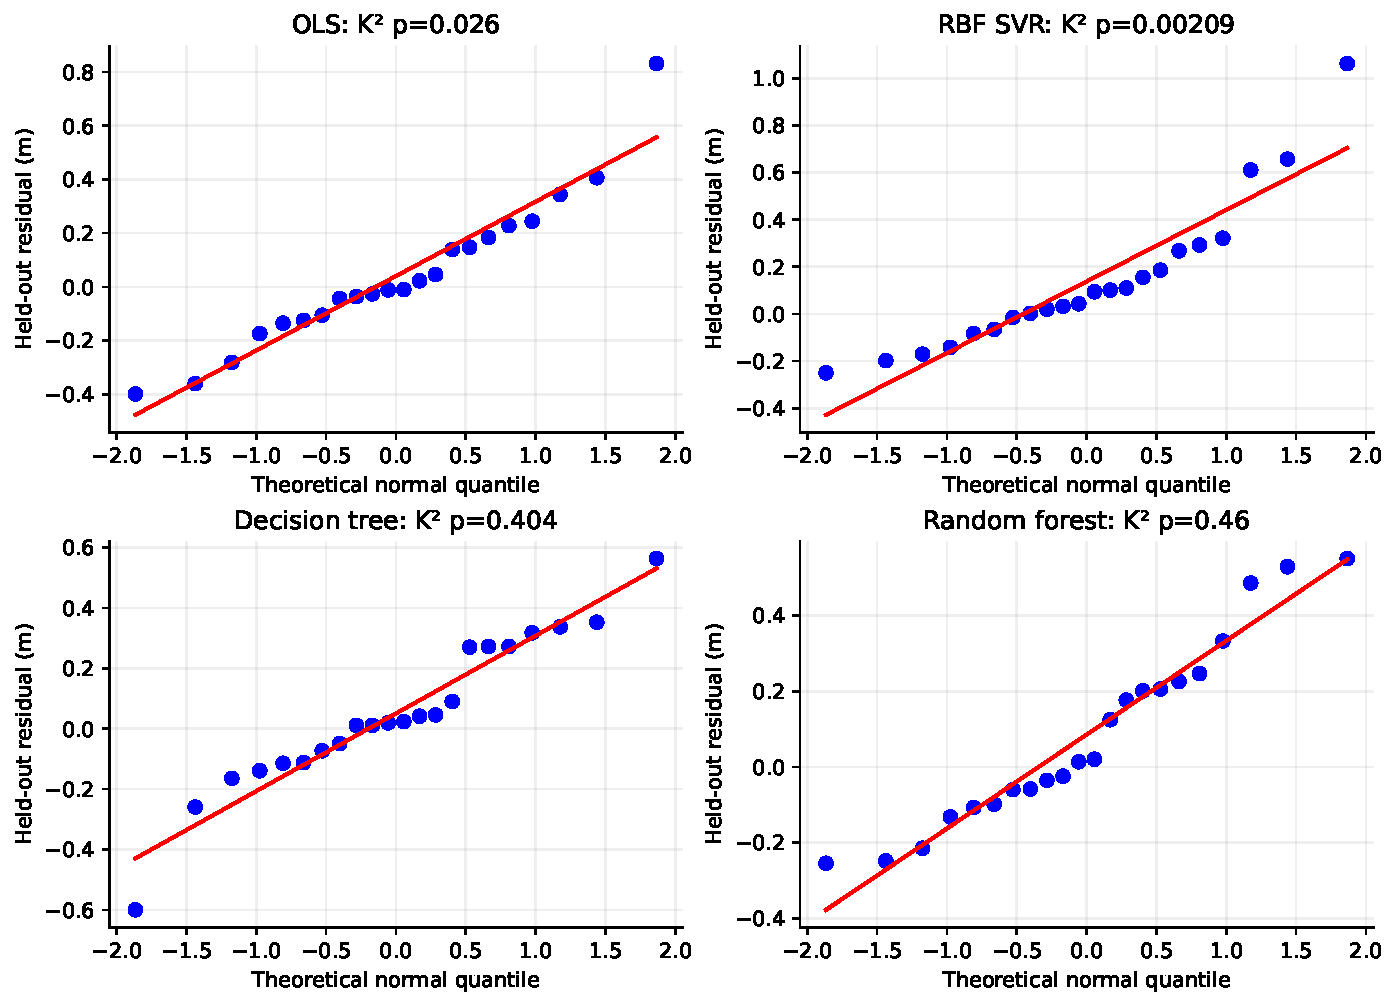
\includegraphics[width=.98\linewidth]{results/figures/q4_qqplots.pdf}
\end{center}
\small
\textbf{Figure 1.} Normal Q--Q plots of held-out ALE residuals. The reference line
is fitted by SciPy's \code{probplot}; straight-line behavior is expected for a
normal distribution after allowing location and scale. Titles show unadjusted
omnibus p-values, not the Holm-adjusted values.
\normalsize
\begin{center}
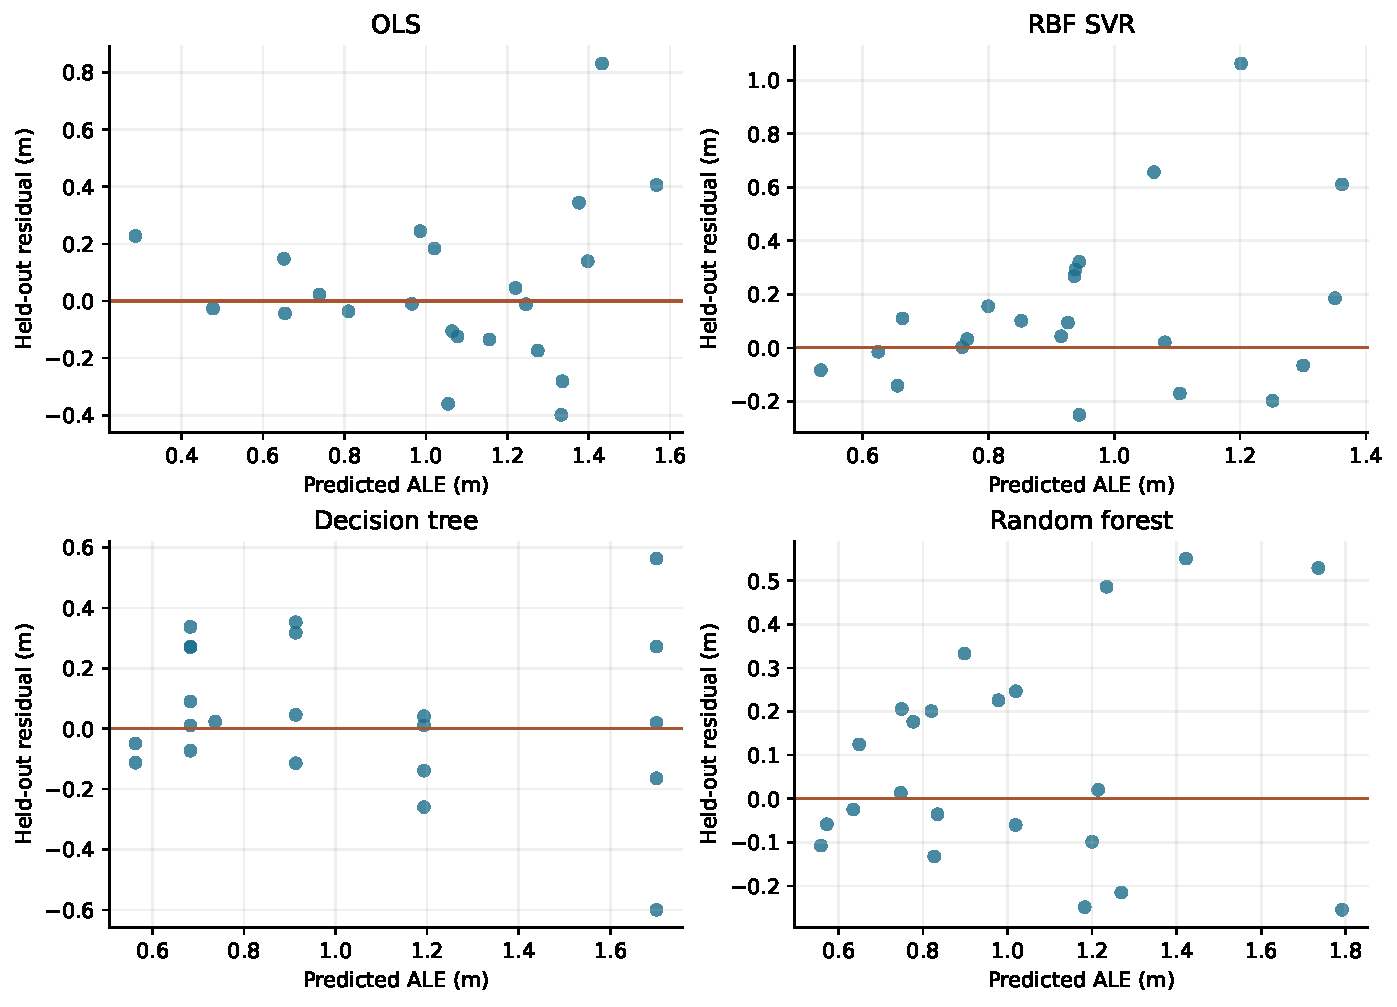
\includegraphics[width=.92\linewidth,height=2.8in,keepaspectratio]{results/figures/q4_residuals.pdf}
\end{center}
\small
\textbf{Figure 2.} Residuals versus predicted ALE on the same test observations.
Departures can reflect model mismatch as well as error-distribution shape.
\normalsize

\newpage
\section*{5. Automatic differentiation: classification}
\subsection*{Common setup and sklearn baseline}
I load Breast Cancer Wisconsin (Diagnostic) using sklearn's
\code{load\_breast\_cancer}: 569 observations and 30 features [2]. Labels are
0=malignant and 1=benign. The 80/20 split is stratified, with seed 42,
giving 455 training and 114 test observations. Inputs are standardized using
training means and standard deviations. The baseline is sklearn
\code{LogisticRegression(C=1, solver="lbfgs", max\_iter=10000, tol=1e-10)}.
It retains default L2 regularization [5].

\subsection*{(a) Logistic model and binary cross-entropy}
The PyTorch affine model computes $z_i=w^T\widetilde x_i+b$ and
$p_i=\sigma(z_i)$. I implement the requested mean BCE as
\[
\mathcal L_{\rm logit}(w,b)
=\frac1n\sum_i\operatorname{softplus}((1-2y_i)z_i),
\qquad \operatorname{softplus}(z)=\log(1+e^z).
\]
For binary labels, this equals both $\operatorname{softplus}(z)-yz$ and
$-y\log p-(1-y)\log(1-p)$. The signed-margin form avoids subtracting nearly
equal large numbers for confidently correct predictions. Stable softplus also
avoids overflow; clipping is unnecessary. Gradients use \code{loss.backward()}.

\subsection*{(b) Probit model with the same BCE}
For probit, $p_i=\Phi(z_i)$. Since $1-\Phi(z)=\Phi(-z)$, the same BCE is
\[
\mathcal L_{\rm probit}(w,b)
=-\frac1n\sum_i\big[y_i\log\Phi(z_i)+(1-y_i)\log\Phi(-z_i)\big].
\]
I use \code{torch.special.log\_ndtr} for stable log-CDF values [6] and
\code{torch.special.ndtr} for probabilities. This avoids losing gradients through
hard probability clipping in the tails.

\subsection*{Training and comparison}
Both custom models use float64 CPU tensors, zero initial weights and bias,
minibatches of 32, random reshuffling, and \code{torch.optim.SGD} with no momentum
or weight decay. In epoch $e=0,1,\ldots$, the learning rate is
$0.05/(1+e/500)$. A further stratified split of the training set (364 inner
training, 91 validation; seed 43) selects the minimum validation BCE among
checkpoints every 10 epochs, up to 2,000. Scaling is refitted on the inner
training subset for this step. Each final model is then trained from scratch
on all 455 training examples for its selected epoch count. Test data are never
used for this choice. Predictions use $p\ge0.5$ for class 1.

\begin{center}\small
\begin{tabular}{lrrr}
\toprule
Model & Correct / test & Accuracy & SGD epochs \\
\midrule
sklearn logistic (L2) & 112/114 & 98.25\% & -- \\
PyTorch logistic & 111/114 & 97.37\% & 80 \\
PyTorch probit & 111/114 & 97.37\% & 20 \\
\bottomrule
\end{tabular}

\end{center}
Each custom classifier makes one more test error than the baseline, a difference
of about 0.88 percentage points. The two custom links tie in accuracy on this
split. This is not evidence of a general performance ranking: the test set is
small, the baseline uses explicit L2 regularization, and the custom models use
unpenalized BCE with early stopping. The comparison therefore includes these
training differences as well as the link function. Saved confusion matrices
and predictions permit a more detailed inspection.

\newpage
\section*{5. Automatic differentiation: regression}
\subsection*{Baseline and (a) squared-error model}
Using the same 85/22 ALE split as Problem 4, the baseline is sklearn
LinearRegression with an intercept. The PyTorch model is
$\widehat y_i=w^T\widetilde x_i+b$, trained by minimizing
\[
\mathcal L_{\rm MSE}(w,b)=\frac1n\sum_i(y_i-w^T\widetilde x_i-b)^2.
\]
This uses the lecture's convention without a factor $1/2$.
Only inputs are standardized; targets remain in their original units.

\subsection*{(b) Student-t residual likelihood}
For $r_i=y_i-\widehat y_i$ and the assigned $\nu=5$, unit-scale density,
\begin{align*}
p(r_i)&=\frac{\Gamma(3)}{\sqrt{5\pi}\,\Gamma(5/2)}
\left(1+\frac{r_i^2}{5}\right)^{-3},\\
\mathcal L_t(w,b)&=\frac1n\sum_i\left[
\tfrac12\log(5\pi)+\log\Gamma(5/2)-\log\Gamma(3)
+3\log\left(1+\frac{r_i^2}{5}\right)\right].
\end{align*}
The implementation uses the negative mean of
\code{StudentT(df=5, loc=0, scale=1).log\_prob(residual)} [7].
The degrees of freedom and scale are fixed, not fitted. In particular, rescaling
$y$ before applying a unit-scale density would change the assigned loss, so I do
not do that.

For a single example,
\[
\frac{\partial L_t}{\partial\widehat y_i}
=-\frac{6r_i}{5+r_i^2},\qquad
\frac{\partial L_{\rm MSE}}{\partial\widehat y_i}=-2r_i.
\]
The Student-t gradient downweights large residuals, while the MSE gradient grows
linearly. This explains robustness to large errors, but does not guarantee a lower
MAE on every test set. The Student-t loss has negative second derivative when
$|r|>\sqrt5$, so the objective is not globally convex in general.

\subsection*{Training, results, and optimization checks}
Both custom regressions use zero initial weights, bias initialized to the training
mean of ALE, 5,000 epochs, minibatches of 16, and ordinary SGD with rate
$0.02/(1+e/100)$. Settings are fixed without test tuning. Primary evaluation is
test mean absolute error, $n_{\rm test}^{-1}\sum_j|y_j-\widehat y_j|$.

\begin{center}\small
\begin{tabular}{lrrr}
\toprule
Model & Test MAE (m) & Test RMSE (m) & Train MSE \\
\midrule
sklearn OLS & 0.195393 & 0.270543 & 0.050582 \\
PyTorch linear, MSE & 0.195373 & 0.270370 & 0.050582 \\
PyTorch linear, Student-t & 0.194071 & 0.272702 & 0.050627 \\
\bottomrule
\end{tabular}

\end{center}
The custom MSE fit nearly reproduces OLS: its training MSE is only
\MSEExcess\ above the OLS optimum, and the largest test-prediction difference
is \PredictionGap\ meters. Small test-MAE differences here are optimization
error, not a change in model class or loss.

Student-t regression lowers test MAE by \StudentImprovement\ meters
(\StudentPercent\%) relative to OLS on this split, while its RMSE is slightly
higher. Thus it trades a small improvement in average absolute error for worse
squared-error performance here. Its training negative log-likelihood is
\TExcess\ above an independent BFGS reference solution. That reference only
checks optimization; all reported model predictions come from SGD. The small
MAE improvement on 22 test observations should not be presented as established
statistical superiority.

\newpage
\section*{Optimization diagnostics and reproducibility}
\begin{center}
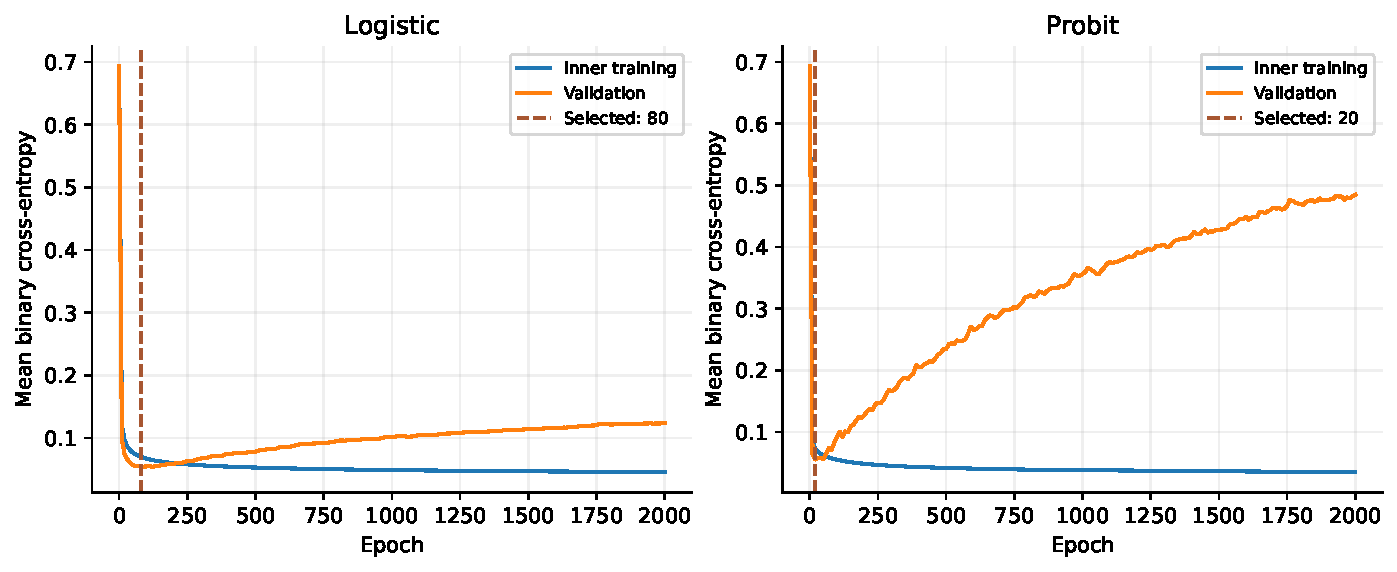
\includegraphics[width=\linewidth]{results/figures/q5_classification_learning.pdf}
\end{center}
\small
\textbf{Figure 3.} Training-only classification epoch selection. Vertical lines
mark the chosen epochs before refitting on the entire training set.
\normalsize
\begin{center}
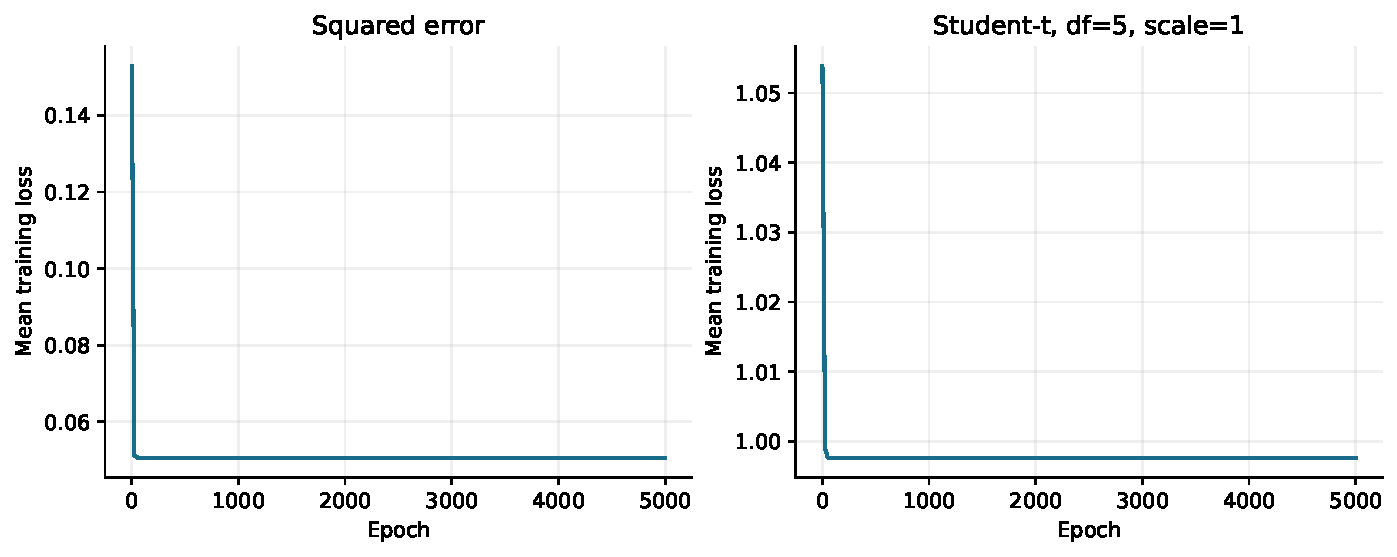
\includegraphics[width=\linewidth]{results/figures/q5_regression_learning.pdf}
\end{center}
\small
\textbf{Figure 4.} Mean training objectives for the two ALE regressions. The
vertical scales differ because the losses have different definitions.
\normalsize

\newpage
\section*{Code access and reproduction}
\textbf{Course repository (clickable):}\\
\url{https://github.com/richard0525/foundations-machine-learning-ai}

\textbf{Homework 1 directory (clickable):}\\
\url{https://github.com/richard0525/foundations-machine-learning-ai/tree/main/homework_1}

The course repository organizes assignments as \code{homework\_1/},
\code{homework\_2/}, and so on as they are completed. This submission contains
\code{homework\_1/}. Its README documents the methods, inputs, and output files.

\subsection*{Clone and run}
With Git and Python 3.12 installed, run these commands from a terminal
(macOS/Linux):
\begin{quote}\small
\begin{verbatim}
git clone https://github.com/richard0525/foundations-machine-learning-ai.git
cd foundations-machine-learning-ai
python3.12 -m venv .venv
.venv/bin/python -m pip install -r homework_1/requirements.txt
.venv/bin/python homework_1/run.py
.venv/bin/python -m unittest discover -s homework_1 -v
.venv/bin/python homework_1/build_report.py
\end{verbatim}
\end{quote}
On Windows, create the environment with \code{py -3.12 -m venv .venv} and
replace \code{.venv/bin/python} with \code{.venv\textbackslash Scripts\textbackslash python.exe}.
No GPU is needed. Dependency installation requires internet access. The ALE CSV
is bundled and checksum-verified; if missing, it is downloaded automatically.
The classification data are bundled with scikit-learn. No data-service account,
API key, or local absolute path is required by the computations.

\subsection*{Expected outputs and verification}
\code{run.py} regenerates the numerical results and plots in
\code{homework\_1/results/}. The saved classification accuracies are 98.25\%
(sklearn logistic) and 97.37\% (both custom classifiers); regression MAEs are
approximately 0.195393, 0.195373, and 0.194071 meters for OLS, MSE SGD, and
Student-t SGD. See the earlier tables for interpretation.

The test command checks custom losses, analytic and finite-difference gradients,
tail stability, data integrity, and recovery of a known linear solution.
There are nine tests. \code{build\_report.py} refreshes the report tables from
the default results directory and rebuilds this PDF if \code{pdflatex} is installed.
LaTeX is optional for running the experiments: the completed PDF is included at
\href{https://github.com/richard0525/foundations-machine-learning-ai/blob/main/homework_1/results/solution.pdf}{\code{homework\_1/results/solution.pdf}}.
All settings in \code{config.json} are part of the reported experiment.

\textbf{Audit trail.} JSON files record fixed seeds, train/test and validation
indices, original and standardized coefficients, preprocessing statistics,
package versions, source hashes, and the data checksum. CSV files expose
per-observation predictions and optimization histories. Runs use one CPU thread
and float64. Dependencies are pinned; tiny floating-point differences across
platforms remain possible. No external credentials are required to run the code.

\newpage
\section*{References}
\small
\begin{enumerate}
\item Singh, A., Kotiyal, V., Sharma, S., Nagar, J., and Lee, C. (2020).
\emph{Average Localization Error (ALE) in sensor node localization process in
WSNs}. UCI Machine Learning Repository.
\href{https://doi.org/10.24432/C5ZP6R}{doi:10.24432/C5ZP6R}.
The public CSV is redistributed unchanged under CC BY 4.0, with its filename
shortened to \code{ale.csv}.
\item Wolberg, W., Mangasarian, O., Street, N., and Street, W. (1993).
\emph{Breast Cancer Wisconsin (Diagnostic)}. UCI Machine Learning Repository.
\href{https://doi.org/10.24432/C5DW2B}{doi:10.24432/C5DW2B}.
Loaded through sklearn's bundled dataset.
\item SciPy. \href{https://docs.scipy.org/doc/scipy/reference/generated/scipy.stats.normaltest.html}{\code{scipy.stats.normaltest}}:
D'Agostino--Pearson omnibus normality test.
\item SciPy. \href{https://docs.scipy.org/doc/scipy/reference/generated/scipy.stats.probplot.html}{\code{scipy.stats.probplot}}:
probability-plot construction and fitted reference line.
\item scikit-learn.
\href{https://scikit-learn.org/stable/modules/generated/sklearn.linear_model.LogisticRegression.html}{\code{LogisticRegression}}:
default regularization and solver parameters.
\item PyTorch.
\href{https://docs.pytorch.org/docs/2.14/special.html}{\code{torch.special}}:
normal CDF and stable log-CDF functions.
\item PyTorch.
\href{https://docs.pytorch.org/docs/2.14/distributions.html}{\code{torch.distributions.StudentT}}:
Student-t log probability with specified degrees of freedom, location, and scale.
\item PyTorch.
\href{https://docs.pytorch.org/docs/2.14/generated/torch.optim.SGD.html}{\code{torch.optim.SGD}}:
stochastic gradient descent optimizer.
\item Veitch, V. Course materials supplied with this assignment:
\emph{Lecture 1}; \emph{Supervised Learning Continued};
\emph{First Look at Generalization}; \emph{Feature Engineering and Deep Learning};
and \emph{Homework 1}, Fall 2026. The theoretical arguments use the notation
and risk-minimization framework of these lectures.
\end{enumerate}
\end{document}
